\def\CLASSINPUTbaselinestretch{2}
\documentclass[12pt,journal,draftclsnofoot,onecolumn,letterpaper]{IEEEtran}
\usepackage[T1]{fontenc}
\usepackage{amsmath,amssymb,graphicx,booktabs,cite,url}
\usepackage[hidelinks]{hyperref}
\hypersetup{pdftitle={NeST-Com: Fixed-Budget Next-Scale Token Communication},pdfauthor={Anonymous Authors}}
\graphicspath{{figures/}}
\newcommand{\Dc}{D_c}
% Allow the tall, double-spaced evidence table near its first citation.
\let\originaltable\table
\renewcommand{\table}[1][t]{\originaltable[!htbp]}
\emergencystretch=3em
\widowpenalty=10000
\clubpenalty=10000
\begin{document}
\title{NeST-Com: Fixed-Budget Next-Scale Token Communication}
\author{Anonymous Authors}
\maketitle
\begin{abstract}
Next-scale residual tokens provide a coarse-to-fine image description, but whole-scale endpoints can underfill fixed digital frames. NeST-Com fits independently terminated, entropy-coded within-scale prefixes to fixed frames and uses received tokens for residual reconstruction and finer-scale conditioning. With shared model components, it improves PSNR over whole-scale transmission by 0.32--0.70~dB at 1024 symbols and 0.39--0.79~dB at 512 symbols. At 1024 symbols and 10~dB, source-bit utilization increases from 77.70\% to 95.21\%. Comparisons with existing systems show favorable low-budget source reconstruction and metric-dependent perceptual tradeoffs.
\end{abstract}
\begin{IEEEkeywords}
Image communication, visual autoregressive models, fixed symbol budget, entropy coding.
\end{IEEEkeywords}

\section{Introduction}
A fixed per-image channel-symbol budget limits the source description available for reconstruction. Feasibility depends on image-dependent source-code length and in-frame protection. A generative prior completes untransmitted information, constrained by the delivered description.

Digital coding and learned joint source--channel coding (JSCC) offer different solutions~\cite{deepjscc,swinjscc}; fitting progressive descriptions to channel resources is a classical problem~\cite{chande}. Ada-TokenCom combines prefix entropy coding, tail generation, and prefix/MCS selection under an average resource constraint~\cite{adatokencom}. TONIC addresses task-oriented token transmission~\cite{tonic}, and ARPC uses next-scale progressive coding~\cite{arpc}. We adopt visual autoregressive modeling (VAR), which reported state-of-the-art results in its original class-conditional ImageNet generation benchmarks~\cite{var}. Its complete coarse maps describe the full latent grid after resizing; later maps add residual refinements. This organization motivates transmitting a limited coarse-to-fine description for source-constrained reconstruction.

Whole-scale boundaries need not align with frame capacity: a complete scale adds many tokens, and its terminated code length varies across images. Within-scale endpoints use capacity left after the last feasible whole scale. Both ends construct matching coding probabilities from complete coarse maps. The received boundary tokens must then enter residual accumulation and the conditions for finer-scale prediction.

NeST-Com combines within-scale endpoints, independently terminated arithmetic streams, actual-length fitting, and prefix-constrained reconstruction. It uses VAR's known-token overwrite~\cite{var} to merge received boundary positions with predictions and update both residual latent and finer-scale context. Shared-model comparisons show 0.32--0.70~dB PSNR gains over whole-scale transmission at $N=1024$ and 0.39--0.79~dB at $N=512$. Controlled endpoint and receiver interventions examine the design, while six-system comparisons and separately calibrated reduced-budget results characterize complete-system quality tradeoffs.

\section{Proposed NeST-Com Framework}
\subsection{Next-Scale Representation and Digital Frame}
We transmit $x\in[0,1]^{256\times256\times3}$ over complex AWGN,
\begin{equation}
 y=s+n,\quad n\sim\mathcal{CN}(0,\sigma^2 I_N),\quad
 \mathrm{SNR}=10\log_{10}(E_s/\sigma^2),
 \label{eq:channel}
\end{equation}
using $N$ complex symbols per image and nominal $E_s=2$. TX selects a frozen policy for the channel SNR; RX uses the true noise variance for LLRs. Digital constellations have average energy two without per-frame renormalization. Continuous JSCC data are normalized per image to average energy two, with required Swin side information paid within $N$. A 12-bit profile ID, CRC16, and terminated rate-1/2 convolutional code occupy 68 rotated-BPSK symbols $\{\pm(1+j)\}$. The remaining $N-68$ symbols carry the LDPC-coded body. The paid profile identifies the actual endpoint and MCS. Our main budget is $N=1024$; the reduced-budget experiment uses $N=512$ without increasing $E_s$.

The frozen VAR tokenizer produces ten residual token maps $q_s$, with side lengths $(1,2,3,4,5,6,8,10,13,16)$ and a 4096-entry codebook~\cite{var}. Let $L_s$ be the map size and $C_s$ its codebook lookup, resizing, and residual transform. Complete coarse maps span the whole latent grid after resizing; the sum $f_q=\sum_s C_s(q_s)$ accumulates their residual refinements. Image decoder $\Dc$ is adapted on 20\,000 ImageNet training images using continuous, fully quantized, and prefix-completion-interpolated latents, then fixed. NeST-Com uses null-class conditioning. Its frozen next-scale prior factorizes as
\begin{equation}
 p_\theta(q_s\mid q_{<s})=\prod_{i=1}^{L_s}p_\theta(q_{s,i}\mid q_{<s}),
 \label{eq:prior}
\end{equation}
providing local cumulative distribution functions (CDFs) for arithmetic coding~\cite{arithmetic} at both ends of Fig.~\ref{fig:system}.

\begin{figure*}[t]
\centering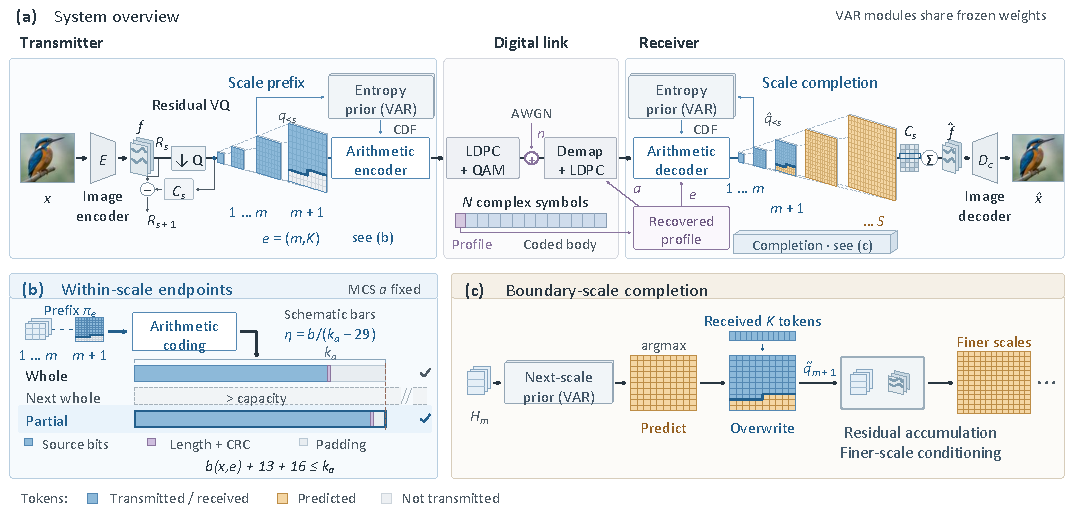
\includegraphics[width=\textwidth]{figure1.pdf}
\caption{NeST-Com. (a) The protected profile specifies the endpoint and MCS; both terminals reconstruct coding probabilities from the shared frozen VAR and their known coarse tokens. (b) Independently terminated within-scale prefixes fit the body capacity; bars are schematic. (c) Received boundary tokens overwrite predicted positions. The merged map updates the residual latent and the context for finer-scale prediction. Unreceived boundary positions retain their coarse-conditioned predictions.}
\label{fig:system}
\end{figure*}

\subsection{Within-Scale Endpoints and Actual-Length Fitting}
An endpoint $e=(m,K)$ retains complete coarse maps and $K$ raster-ordered positions from the next map:
\begin{equation}
 \pi_e=(q_1,\ldots,q_m,q_{m+1,1:K}).
 \label{eq:prefix}
\end{equation}
WHOLE permits $K=0$ for $m=4,\ldots,10$. PARTIAL adds
$K\in\{\lfloor L_{m+1}/4\rfloor,\allowbreak\lfloor L_{m+1}/2\rfloor,\allowbreak\lfloor3L_{m+1}/4\rfloor\}$ for $m=4,\ldots,9$, giving 25 endpoints in total. $(10,0)$ is the full representation.

For MCS $a=(M,r)$, the coded body has $n_a=(N-68)\log_2M$ bits and information length $k_a=\lfloor rn_a\rfloor$. With actual terminated arithmetic length $b(x,e)$,
\begin{equation}
 b(x,e)+29\leq k_a,\qquad \eta(x,e)=\frac{b(x,e)}{k_a-29}.
 \label{eq:budget}
\end{equation}
The endpoint specifies retained source tokens; its actual terminated length determines frame feasibility. The 29 bits comprise the 13-bit length field and CRC16; unused information positions are zero-padded before 5G NR LDPC coding, rate matching~\cite{nr}, and QAM. Thus $\eta$ measures source-bit capacity utilization, not total over-the-air efficiency.

Offline calibration selects a target endpoint and MCS for each budget/SNR. A 100-image pilot uses one channel realization per image; the finalists are evaluated on all 1000 calibration images with three realizations per image. Selection maximizes source/reconstruction DINOv2 cosine~\cite{dinov2}, averaged over realizations first and then equally over sources, including gray failures. Exact ties use a fixed candidate order. At $N=1024$, target screening starts at scales 7--9 and includes full-scale $(10,0)$ candidates in final evaluation. At $N=512$, WHOLE/PARTIAL screen all 7/25 targets against the same 12 MCSs, $\log_2M\in\{2,4,6\}$ and $r\in\{1/2,2/3,3/4,5/6\}$. Each method/SNR advances the top three plus a maximum-endpoint QPSK rate-1/2 anchor. Ada uses the same N512 MCS pool with longest-feasible fitting up to 256 tokens. The full candidate and selection rules are provided with the results.

Online fitting fixes the selected MCS and searches legal endpoints no longer than the target, in decreasing token count down to $(4,0)$. TX sends the first independently terminated stream satisfying~\eqref{eq:budget}; the paid profile identifies the actual endpoint. Arithmetic streams are never cut from longer streams. If no endpoint fits, the N512 protocol sends a paid NULL profile and short NULL payload through the complete frame, retaining a gray reconstruction in the denominator. The N1024 implementation instead raises an error; no evaluated N1024 source encountered this case.

\subsection{Prefix-Constrained Reconstruction}
Invalid profile CRC/catalogue, body CRC, declared length, known padding, or arithmetic parsing produces a fixed gray image; so does a valid N512 NULL reception. Otherwise, RX decodes the prefix using CDFs rebuilt from received complete coarse maps. It predicts the boundary map by VAR argmax conditioned on those maps, then applies known-token overwrite~\cite{var}:
\begin{equation}
 \tilde q_{m+1,i}=\begin{cases}\hat q_{m+1,i},&i\leq K,\\q^{\mathrm{pred}}_{m+1,i},&i>K.\end{cases}
 \label{eq:overwrite}
\end{equation}
Unreceived boundary positions retain their coarse-conditioned prediction. Received boundary tokens serve two roles: they correct the residual representation and, through the merged boundary map, condition the prediction of finer scales. Complete received maps remain unchanged; subsequent maps are generated from this updated context. Reconstruction is
\begin{equation}
 \hat x=\Dc\!\left(\sum_{s=1}^{10}C_s(\tilde q_s)\right).
 \label{eq:reconstruction}
\end{equation}
At the final scale, overwrite changes the residual contribution without any subsequent propagation.

\section{Experimental Results}
\begin{figure*}[t]
\centering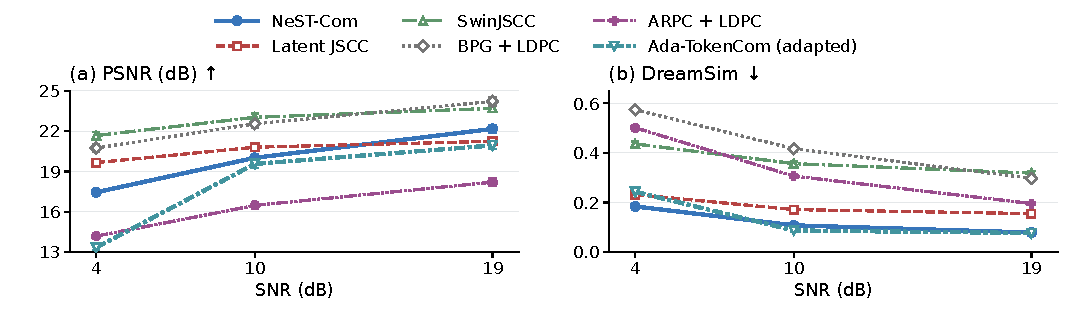
\includegraphics[width=\textwidth]{figure2.pdf}
\caption{Six-system performance on common500 at $N=1024$. Points and error bars are equal-source means and pointwise 95\% source-bootstrap confidence intervals after averaging three channel realizations per source. Ada denotes the predicted-class, fixed-frame adaptation. Higher PSNR and lower DreamSim are favorable.}
\label{fig:performance}
\end{figure*}
\subsection{Experimental Setup}
We use common500 ImageNet validation images~\cite{imagenet}, a disjoint cal1000 set, and Kodak24~\cite{kodak}, with fixed $256\times256$ preprocessing. ImageNet-calibrated policies remain fixed on Kodak. The six-system main study uses $N=1024$; NeST, WHOLE, and Ada also use $N=512$, each independently calibrated at 4/10/19~dB.

Our convolutional Latent JSCC maps tokenizer latents to symbols and shares $\Dc$, using MSE, LPIPS, and latent-consistency losses. It and SwinJSCC~\cite{swinjscc}, adapted to $256\times256$ and $N=1024$, use the same 20\,000 training images and final 100k/200k-update checkpoints. SwinJSCC was still improving at its training cap. Digital baselines are adaptive BPG~\cite{bpg} + LDPC, ARPC~\cite{arpc} + LDPC with paid captions, and predicted-class, fixed-frame Ada~\cite{adatokencom}. Ada retains LlamaGen-L/VQ16 and prefix arithmetic coding. A fixed ConvNeXt predicts the paid 10-bit class ($b+39\leq k_a$); fitting searches all 1--256-token endpoints. Its tail uses CFG=4, $T=1$, top-$k=2000$, top-$p=1$. This adaptation does not reproduce Ada's average-budget controller or ARQ.

Metrics are PSNR, LPIPS-Alex~\cite{lpips}, DreamSim~\cite{dreamsim}, and CLIP ViT-L/14 image--image cosine (CLIP-I)~\cite{clip}. Frozen FP32 preprocessing uses $224\times224$ bicubic-antialias inputs for DreamSim/CLIP. DINOv2-based calibration is related to feature-based evaluation; controlled interventions provide the mechanism evidence. Three original channel outcomes, including gray failures, are averaged per source before equal-source means and direct source-paired 95\% bootstrap intervals (10\,000 resamples). N512 shares source/repeat-specific AWGN across methods; N1024 retains historical noise identities. E1/E2 use the fixed existing 100-source subset and actual received inputs, without new PHY trials or training. They are diagnostics, not new independent test sets.

\subsection{Effect of Within-Scale Endpoints}
\begin{table}[t]
\caption{Within-scale endpoint and receiver evidence. (A) Main family-specific policies; differences are PARTIAL minus WHOLE. (B) Controlled granularity on 100 sources with fixed model, MCS, maximum endpoint and fitting rule. (C) Receiver interventions on the same 100 sources and actual prefixes. Brackets give source-paired 95\% CIs; populations and conditions are as stated.}
\label{tab:internal}
\centering\footnotesize
\setlength{\tabcolsep}{2.5pt}
\begin{tabular}{ccc}
\toprule
\multicolumn{3}{l}{(A) Main policies at $N=1024$} \\
SNR & Util. W$\to$P (\%) & $\Delta$PSNR (dB) [95\% CI] \\
\midrule
\multicolumn{3}{l}{common500} \\
4 & 73.81 $\to$ 93.08 & $+0.616\;[0.564,0.673]$ \\
10 & 77.70 $\to$ 95.21 & $+0.701\;[0.637,0.766]$ \\
19 & 85.24 $\to$ 94.73 & $+0.319\;[0.290,0.349]$ \\
\multicolumn{3}{l}{Kodak24} \\
4 & 75.69 $\to$ 93.43 & $+0.396\;[0.236,0.543]$ \\
10 & 78.11 $\to$ 94.99 & $+0.674\;[0.408,0.958]$ \\
19 & 85.69 $\to$ 93.71 & $+0.228\;[0.140,0.324]$ \\
\midrule
\multicolumn{3}{l}{(B) Fixed-granularity diagnostic, 10 dB} \\
Grid (candidates) & Utilization (\%) & PSNR (dB) \\
Whole (7) & 78.15 & 18.952 \\
Half (13) & 89.21 & 19.396 \\
Quarter (25) & 95.38 & 19.612 \\
Eighth (49) & 97.39 & 19.735 \\
\midrule
\multicolumn{3}{l}{(C) Receiver interventions: $\Delta$PSNR (dB) [95\% CI]} \\
SNR & B0$-$A0 & C0$-$B0 \\
10 & $+0.220\;[0.176,0.264]$ & $+0.440\;[0.330,0.558]$ \\
19 & $+0.301\;[0.247,0.358]$ & $+0.000\;[0.000,0.000]$ \\
\bottomrule
\end{tabular}
\end{table}

Table~\ref{tab:internal}(A) compares WHOLE/PARTIAL with shared tokenizer, prior, entropy coder, and $\Dc$. Separate family calibration selects the same MCS at each SNR. Common500 gains are 0.32--0.70~dB PSNR. At 10~dB, source-bit utilization rises from 77.70\% to 95.21\% and DreamSim falls by 0.0240. Kodak gains 0.674~dB and reduces DreamSim by 0.0164; its 19~dB DreamSim interval includes zero.

Block~B fixes the 100 sources, model, MCS, maximum endpoint, and fitting rule. Eighth adds $0.123\,[0.079,0.169]$~dB over Quarter at 10~dB, but its DreamSim/CLIP-I difference intervals cross zero. Mean terminated-length checks increase from 3.55/5.55/9.49 to 17.58 for Whole/Half/Quarter/Eighth. These checks compare terminated streams, not model forwards or elapsed time; Quarter is predefined.

Block~C uses the same actual prefixes. A0 ignores received boundary tokens and follows the prior. B0 adds their correction to the final residual latent while finer-scale conditioning follows A0. C0 updates both latent and conditioning, on the same device and precision. The ordered PSNR differences are 0.220 and 0.440~dB at 10~dB. At 19~dB, the last-scale boundary leaves no C0$-$B0 increment. A0 still uses completion; these diagnostics do not decompose the common500 gain.

E2 separately compares direct coarse decoding, $R0=\Dc(\sum_{s=1}^{m}C_s(q_s))$, with existing VAR-completed WHOLE output R1 from the identical received prefix. Both retain the original ten-scale transforms, full latent grid, and frozen $\Dc$. R1$-$R0 PSNR is $0.026\,[-0.204,0.271]$~dB at N512, 4~dB, and $0.771\,[0.563,0.986]$~dB at 10~dB. DreamSim changes by $-0.4204\,[-0.4488,-0.3925]$ and $-0.4519\,[-0.4790,-0.4248]$, respectively; LPIPS decreases and CLIP-I increases at both points with intervals excluding zero. Thus completion improves feature quality here, while its PSNR benefit depends on the operating point and adapted decoder.

\subsection{Comparison With Existing Methods}
\begin{table}[t]
\caption{Perceptual distance and image-feature similarity on common500 at $N=1024$. Each cell is LPIPS-Alex$\downarrow$ / CLIP-I$\uparrow$. Ada denotes the fixed-frame adaptation. Values are source means.}
\label{tab:external}
\centering\footnotesize
\setlength{\tabcolsep}{3pt}
\begin{tabular}{lccc}
\toprule Method & 4 dB & 10 dB & 19 dB \\
\midrule
NeST-Com & 0.263 / 0.821 & 0.171 / 0.873 & 0.118 / 0.900 \\
Latent JSCC & 0.219 / 0.741 & 0.173 / 0.789 & 0.158 / 0.804 \\
SwinJSCC & 0.530 / 0.627 & 0.469 / 0.669 & 0.440 / 0.697 \\
BPG + LDPC & 0.725 / 0.586 & 0.589 / 0.635 & 0.458 / 0.684 \\
ARPC + LDPC & 0.512 / 0.644 & 0.341 / 0.713 & 0.250 / 0.788 \\
Ada (adapted) & 0.395 / 0.828 & 0.167 / 0.884 & 0.138 / 0.892 \\
\bottomrule
\end{tabular}
\end{table}

Fig.~\ref{fig:performance} and Table~\ref{tab:external} compare complete systems with different tokenizers, priors, decoders, conditioning, and decoding rules. NeST exceeds Ada in PSNR by 4.116/0.455/1.226~dB at 4/10/19~dB. Ada has better LPIPS, DreamSim, and CLIP-I at 10~dB, higher CLIP-I at 4~dB, and slightly lower DreamSim at 19~dB. At 19~dB Ada transmits all 256 tokens: its approximately 58\% source-capacity utilization reflects a complete representation. SwinJSCC and BPG have higher PSNR than NeST throughout; Latent JSCC has higher PSNR at 4/10~dB and lower LPIPS at 4~dB. NeST's PSNR advantage over ARPC is 3.26--3.97~dB.

E1 changes only Ada's unreceived-tail sampling to argmax, rebuilding context from the received prefix and following the greedy path. At N1024, 10~dB, argmax minus sampling gives $-0.156\,[-0.369,0.057]$~dB PSNR and $+0.0036\,[0.0010,0.0060]$ DreamSim. On these same 100 sources, NeST minus argmax yields $+0.568\,[0.246,0.902]$~dB PSNR but $+0.0178\,[0.0129,0.0229]$ DreamSim; Ada retains higher CLIP-I, while the LPIPS difference interval crosses zero. The original sampling baseline remains in the main comparison.

No rejected or failed reconstructions occurred in the 1500 trials per method at each matched SNR on common500 at N1024. Latent JSCC has no discrete CRC rejection. On Kodak, all four paired metrics favor NeST over Ada at 4~dB; only PSNR excludes zero at 10~dB, and PSNR/LPIPS favor NeST at 19~dB while DreamSim/CLIP-I intervals cross zero.

\subsection{Transmission With a Reduced Symbol Budget}
\begin{figure*}[t]
\centering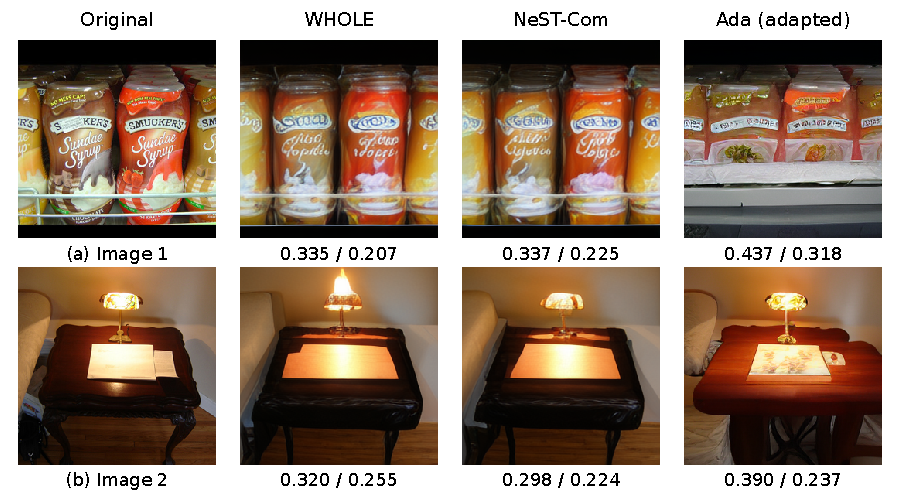
\includegraphics[width=6.0in]{figure3.pdf}
\caption{Source reconstructions at $N=512$ and 10~dB for two images selected by the preregistered source-ID rule. Columns show the original, WHOLE, NeST-Com, and the fixed-frame Ada-TokenCom adaptation. Each reconstruction uses the first registered channel repetition. Values are LPIPS-Alex$\downarrow$ / DreamSim$\downarrow$ for the displayed realization.}
\label{fig:qualitative}
\end{figure*}
\begin{table}[t]
\caption{Reduced-budget comparison on common500 at $N=512$. Differences are NeST-Com minus the fixed-frame Ada-TokenCom adaptation; brackets give source-paired 95\% CIs. Positive PSNR and negative DreamSim favor NeST-Com.}
\label{tab:reduced}
\centering\footnotesize
\setlength{\tabcolsep}{4pt}
\begin{tabular}{ccc}
\toprule SNR & $\Delta$PSNR (dB) & $\Delta$DreamSim \\
\midrule
4 & $+4.180$ & $-0.1029$ \\
 & $[3.991,4.377]$ & $[-0.1142,-0.0917]$ \\
10 & $+4.055$ & $-0.0660$ \\
 & $[3.880,4.235]$ & $[-0.0747,-0.0573]$ \\
19 & $+1.740$ & $+0.0139$ \\
 & $[1.577,1.909]$ & $[0.0103,0.0173]$ \\
\bottomrule
\end{tabular}
\end{table}

At $N=512$, 68 header symbols leave 444 body symbols. WHOLE minus Ada has descriptive PSNR mean differences of 3.79/3.66/0.95~dB at 4/10/19~dB. NeST further improves over WHOLE by $0.392\,[0.341,0.444]$, $0.399\,[0.356,0.445]$, and $0.792\,[0.740,0.844]$~dB; all corresponding LPIPS, DreamSim, and CLIP-I paired intervals also favor NeST. At 10~dB, WHOLE/NeST select the same target $(7,0)$ and 16-QAM rate-2/3 MCS; additional within-scale fallback endpoints raise utilization from 79.30\% to 93.46\%.

NeST has higher PSNR and lower LPIPS than Ada at all three SNRs. DreamSim favors NeST at 4/10~dB and Ada at 19~dB (Table~\ref{tab:reduced}); CLIP-I favors Ada throughout. In Fig.~\ref{fig:qualitative}(a), WHOLE/NeST retain the jar arrangement more closely than Ada, but WHOLE has lower displayed distances than NeST. All methods alter lamp/tabletop details in (b), where NeST has the lowest distances. Individual outcomes differ from the aggregate ranking.

In E1 at N512, argmax reduces Ada PSNR by $0.475\,[0.152,0.801]$ and $0.651\,[0.338,0.984]$~dB at 4/10~dB and worsens all three feature metrics. NeST minus argmax remains $4.632\,[4.183,5.093]$ and $4.600\,[4.188,5.018]$~dB; its LPIPS/DreamSim intervals also favor NeST, while CLIP-I intervals cross zero. This fixed greedy variant preserves the low-budget gap without isolating all model differences.

Main-study body-CRC rejections are 4/7/5 for NeST/WHOLE/Ada at 4~dB, 1/0/0 at 10~dB, and zero at 19~dB, each out of 1500. All remain in the means; no source requires NULL. Independent calibration and different candidate pools preclude attributing cross-budget differences solely to $N$ or representation order.

\subsection{Additional Results and Processing Cost}
At $N=2048$ (100 sources, two paid 1024-symbol subframes), complete representations at 19~dB give NeST $+1.806$~dB PSNR over ARPC, but worse DISTS~\cite{dists}: $+0.0054\,[0.0024,0.0086]$. With WHOLE/PARTIAL policies fixed at 10~dB and true RX noise variance, all 300 receptions per method on 100 sources are rejected at 8~dB; all succeed at 10/12~dB with identical recovered prefixes and images for each source/method.

Mean TX+RX software processing times at 10~dB are 619.71~ms/image for NeST, 42.48 for Latent JSCC, 44.69 for SwinJSCC, 1520.30 for ARPC, and 2293.01 for BPG (RTX PRO~6000, six CPU cores, batch one, 16 development images, three repeats after warm-up). Ada has not been timed under this protocol.

\section{Conclusion}
NeST-Com fits coarse-to-fine residual descriptions to fixed digital frames through within-scale endpoints, actual terminated lengths, and prefix-constrained reconstruction. Shared-model evidence supports improved utilization and reconstruction at both budgets; completion's PSNR benefit depends on the operating point. The low-budget gap to adapted Ada persists under the tested greedy decoder, alongside metric-dependent perceptual tradeoffs. SNR uncertainty remains a limitation and direction for future work.

\begin{thebibliography}{17}
\interlinepenalty=10000
\bibitem{deepjscc} E. Bourtsoulatze, D. B. Kurka, and D. G\"und\"uz, ``Deep joint source-channel coding for wireless image transmission,'' \emph{IEEE Trans. Cogn. Commun. Netw.}, vol. 5, no. 3, pp. 567--579, Sep. 2019.
\bibitem{swinjscc} K. Yang, S. Wang, J. Dai, X. Qin, K. Niu, and P. Zhang, ``SwinJSCC: Taming Swin Transformer for deep joint source-channel coding,'' \emph{IEEE Trans. Cogn. Commun. Netw.}, vol. 11, no. 1, pp. 90--104, Feb. 2025.
\bibitem{chande} V. Chande and N. Farvardin, ``Progressive transmission of images over memoryless noisy channels,'' \emph{IEEE J. Sel. Areas Commun.}, vol. 18, no. 6, pp. 850--860, Jun. 2000, doi: 10.1109/49.848239.
\bibitem{adatokencom} Z. Zhang, L. Qiao, M. B. Mashhadi, Z. Gao, M. Bennis, and K. Huang, ``Ada-TokenCom: Rate-adaptive token communications via large-model-driven token compression and generation,'' 2026, arXiv:2608.28086.
\bibitem{tonic} S. Liu and K. Wang, ``TONIC: Token-centric semantic communication for task-oriented wireless systems,'' 2026, arXiv:2605.21553.
\bibitem{arpc} Z. Zhang, Y. Xia, B. Chen, T. Zhang, H. Wang, and H. Qiu, ``Autoregressive-based progressive coding for ultra-low bitrate image compression,'' in \emph{Int. Conf. Learning Representations}, 2026.
\bibitem{var} K. Tian, Y. Jiang, Z. Yuan, B. Peng, and L. Wang, ``Visual autoregressive modeling: Scalable image generation via next-scale prediction,'' in \emph{Advances in Neural Information Processing Systems}, vol. 37, 2024, pp. 84\,839--84\,865.
\bibitem{arithmetic} I. H. Witten, R. M. Neal, and J. G. Cleary, ``Arithmetic coding for data compression,'' \emph{Commun. ACM}, vol. 30, no. 6, pp. 520--540, Jun. 1987, doi: 10.1145/214762.214771.
\bibitem{nr} 3GPP, ``NR; Multiplexing and channel coding,'' TS 38.212, ver. 16.5.0, Release 16, 2021. [Online]. Available: \url{https://www.etsi.org/deliver/etsi_ts/138200_138299/138212/16.05.00_60/ts_138212v160500p.pdf}
\bibitem{dinov2} M. Oquab \emph{et al.}, ``DINOv2: Learning robust visual features without supervision,'' \emph{Trans. Mach. Learn. Res.}, Jan. 2024. [Online]. Available: \url{https://openreview.net/forum?id=a68SUt6zFt}
\bibitem{imagenet} O. Russakovsky \emph{et al.}, ``ImageNet large scale visual recognition challenge,'' \emph{Int. J. Comput. Vis.}, vol. 115, no. 3, pp. 211--252, 2015.
\bibitem{kodak} R. Franzen, ``Kodak lossless true color image suite,'' accessed Oct. 26, 2026. [Online]. Available: \url{https://r0k.us/graphics/kodak/}
\bibitem{bpg} F. Bellard, ``BPG image format,'' accessed Oct. 22, 2026. [Online]. Available: \url{https://bellard.org/bpg/}
\bibitem{lpips} R. Zhang, P. Isola, A. A. Efros, E. Shechtman, and O. Wang, ``The unreasonable effectiveness of deep features as a perceptual metric,'' in \emph{Proc. IEEE Conf. Comput. Vis. Pattern Recognit.}, Jun. 2018, pp. 586--595.
\bibitem{dreamsim} S. Fu, N. Tamir, S. Sundaram, L. Chai, R. Zhang, T. Dekel, and P. Isola, ``DreamSim: Learning new dimensions of human visual similarity using synthetic data,'' in \emph{Advances in Neural Information Processing Systems}, vol. 36, 2023, pp. 50\,742--50\,768.
\bibitem{clip} A. Radford \emph{et al.}, ``Learning transferable visual models from natural language supervision,'' in \emph{Proc. 38th Int. Conf. Mach. Learn.}, vol. 139, 2021, pp. 8748--8763.
\bibitem{dists} K. Ding, K. Ma, S. Wang, and E. P. Simoncelli, ``Image quality assessment: Unifying structure and texture similarity,'' \emph{IEEE Trans. Pattern Anal. Mach. Intell.}, vol. 44, no. 5, pp. 2567--2581, May 2022.
\end{thebibliography}

\end{document}
